\chapter{Aplicación Meteorológica.}\label{sec:AplicacionMeteorologica}

\paragraph{}En este capítulo se va a exponer el diseño y la arquitectura del software
de la aplicación que usaremos de ejemplo para utilizar el entorno de desarrollo.

\section{Requisitos}

\paragraph{}En esta sección se describirán los requisitos utilizados para el diseño
de la aplicación.

\subsection{Requisitos de sistema:}
\begin{itemize}
    \item El disposivo requerirá acceso a internet para obtener las métricas.
    \item Las métricas deben acualizarse cada 15 minutos.
    \item El sistema debe iniciarse tan pronto como se conecte a una fuente de energía.
    \item La pantalla debe permanecer encendida en todo momento.
\end{itemize}

\subsection{Requisitos de Interfaz:}
\begin{itemize}
    \item La interfaz mostrará la hora en formato 24h.
    \item La interzaz mostrará la fecha, indicando: día de la semana, día del mes, mes y año.
    \item La interfaz mostrará la ubicación utilizada para obtener las métricas.
    \item La interfaz mostrará la situación meteorológica de palabra y con un icono.
    \item La interfaz mostrará la temperatura y la humedad.
    \item La interfaz deberá mostrar siempre los últimos datos optenidos.
    \item La interfaz permitirá el cambio de ubicación mediante uso de la pantalla.
\end{itemize}

\section{Casos de Uso}

\paragraph{}En esta sección se describen los casos de uso extraídos de los requisitos
y que posteriormente se utilizan para el diseño de la arquitectura software.

\section{Interfaz de usuario}

\paragraph{}La interfaz de usuario en este caso se compone únicamente de una pantalla
táctil. Los diseño mostrados en esta sección pertenecen a capturas de pantalla extraidas
de Figma, servicio online de diseño que ha sido elegido para este caso. Por eso mismo
pueden no resultar una muestra exacta del la interfaz final implementada.

\paragraph{}\textbf{Pantalla principal:}

\begin{figure}[H]
	\centering
	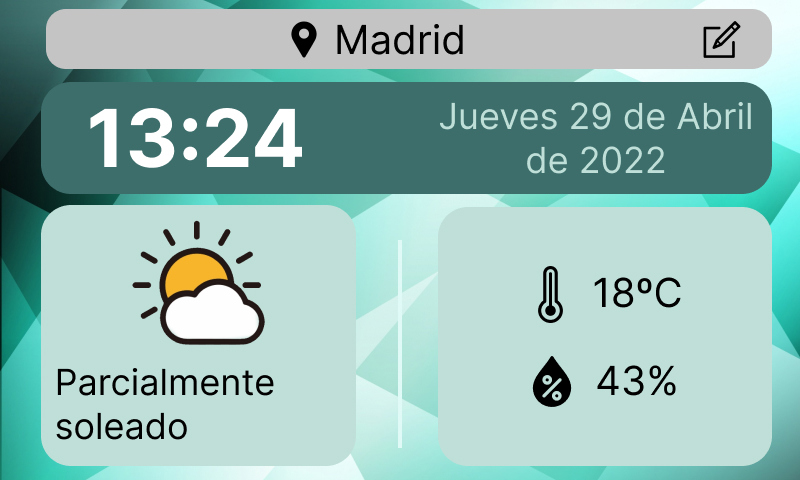
\includegraphics[width=0.75\linewidth]{imgs/figma-main}
	\caption[Diseño de la pantalla principal]{Diseño de la pantalla principal}
	\label{fig:design_main_screen}
\end{figure}

\paragraph{}\textbf{Edición de la localización:}

\begin{figure}[H]
	\centering
	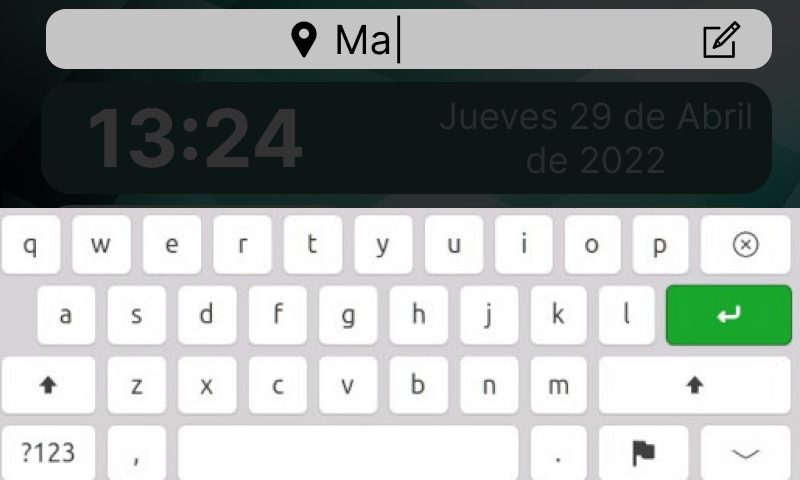
\includegraphics[width=0.75\linewidth]{imgs/figma-location}
	\caption[Diseño del cambio de localización]{Diseño del cambio de localización}
	\label{fig:design_location}
\end{figure}

\section{Arquitectura}

\paragraph{}Blabla

%las referencias a artculos se ponen con \cite,
%las referencias a imgenes \ref,
%las referencias a glosario \gls,
%y las referencias a ecuaciones \eqref
